%% bare_jrnl.tex
%% V1.4b
%% 2015/08/26
%% by Michael Shell
%% see http://www.michaelshell.org/
%% for current contact information.
%%
%% This is a skeleton file demonstrating the use of IEEEtran.cls
%% (requires IEEEtran.cls version 1.8b or later) with an IEEE
%% journal paper.
%%
%% Support sites:
%% http://www.michaelshell.org/tex/ieeetran/
%% http://www.ctan.org/pkg/ieeetran
%% and
%% http://www.ieee.org/

%%*************************************************************************
%% Legal Notice:
%% This code is offered as-is without any warranty either expressed or
%% implied; without even the implied warranty of MERCHANTABILITY or
%% FITNESS FOR A PARTICULAR PURPOSE! 
%% User assumes all risk.
%% In no event shall the IEEE or any contributor to this code be liable for
%% any damages or losses, including, but not limited to, incidental,
%% consequential, or any other damages, resulting from the use or misuse
%% of any information contained here.
%%
%% All comments are the opinions of their respective authors and are not
%% necessarily endorsed by the IEEE.
%%
%% This work is distributed under the LaTeX Project Public License (LPPL)
%% ( http://www.latex-project.org/ ) version 1.3, and may be freely used,
%% distributed and modified. A copy of the LPPL, version 1.3, is included
%% in the base LaTeX documentation of all distributions of LaTeX released
%% 2003/12/01 or later.
%% Retain all contribution notices and credits.
%% ** Modified files should be clearly indicated as such, including  **
%% ** renaming them and changing author support contact information. **
%%*************************************************************************


% *** Authors should verify (and, if needed, correct) their LaTeX system  ***
% *** with the testflow diagnostic prior to trusting their LaTeX platform ***
% *** with production work. The IEEE's font choices and paper sizes can   ***
% *** trigger bugs that do not appear when using other class files.       ***                          ***
% The testflow support page is at:
% http://www.michaelshell.org/tex/testflow/



\documentclass[12pt, technote]{IEEEtran}
%
% If IEEEtran.cls has not been installed into the LaTeX system files,
% manually specify the path to it like:
% \documentclass[journal]{../sty/IEEEtran}




% Some very useful LaTeX packages include:
% (uncomment the ones you want to load)


% *** MISC UTILITY PACKAGES ***
%
%\usepackage{ifpdf}
% Heiko Oberdiek's ifpdf.sty is very useful if you need conditional
% compilation based on whether the output is pdf or dvi.
% usage:
% \ifpdf
%   % pdf code
% \else
%   % dvi code
% \fi
% The latest version of ifpdf.sty can be obtained from:
% http://www.ctan.org/pkg/ifpdf
% Also, note that IEEEtran.cls V1.7 and later provides a builtin
% \ifCLASSINFOpdf conditional that works the same way.
% When switching from latex to pdflatex and vice-versa, the compiler may
% have to be run twice to clear warning/error messages.






% *** CITATION PACKAGES ***
%
%\usepackage{cite}
% cite.sty was written by Donald Arseneau
% V1.6 and later of IEEEtran pre-defines the format of the cite.sty package
% \cite{} output to follow that of the IEEE. Loading the cite package will
% result in citation numbers being automatically sorted and properly
% "compressed/ranged". e.g., [1], [9], [2], [7], [5], [6] without using
% cite.sty will become [1], [2], [5]--[7], [9] using cite.sty. cite.sty's
% \cite will automatically add leading space, if needed. Use cite.sty's
% noadjust option (cite.sty V3.8 and later) if you want to turn this off
% such as if a citation ever needs to be enclosed in parenthesis.
% cite.sty is already installed on most LaTeX systems. Be sure and use
% version 5.0 (2009-03-20) and later if using hyperref.sty.
% The latest version can be obtained at:
% http://www.ctan.org/pkg/cite
% The documentation is contained in the cite.sty file itself.






% *** GRAPHICS RELATED PACKAGES ***
%
\ifCLASSINFOpdf
  % \usepackage[pdftex]{graphicx}
  % declare the path(s) where your graphic files are
  % \graphicspath{{../pdf/}{../jpeg/}}
  % and their extensions so you won't have to specify these with
  % every instance of \includegraphics
  % \DeclareGraphicsExtensions{.pdf,.jpeg,.png}
\else
  % or other class option (dvipsone, dvipdf, if not using dvips). graphicx
  % will default to the driver specified in the system graphics.cfg if no
  % driver is specified.
  % \usepackage[dvips]{graphicx}
  % declare the path(s) where your graphic files are
  % \graphicspath{{../eps/}}
  % and their extensions so you won't have to specify these with
  % every instance of \includegraphics
  % \DeclareGraphicsExtensions{.eps}
\fi
\usepackage{graphicx}  % For including graphics
\usepackage{subcaption}  % For subfigures
% graphicx was written by David Carlisle and Sebastian Rahtz. It is
% required if you want graphics, photos, etc. graphicx.sty is already
% installed on most LaTeX systems. The latest version and documentation
% can be obtained at: 
% http://www.ctan.org/pkg/graphicx
% Another good source of documentation is "Using Imported Graphics in
% LaTeX2e" by Keith Reckdahl which can be found at:
% http://www.ctan.org/pkg/epslatex
%
% latex, and pdflatex in dvi mode, support graphics in encapsulated
% postscript (.eps) format. pdflatex in pdf mode supports graphics
% in .pdf, .jpeg, .png and .mps (metapost) formats. Users should ensure
% that all non-photo figures use a vector format (.eps, .pdf, .mps) and
% not a bitmapped formats (.jpeg, .png). The IEEE frowns on bitmapped formats
% which can result in "jaggedy"/blurry rendering of lines and letters as
% well as large increases in file sizes.
%
% You can find documentation about the pdfTeX application at:
% http://www.tug.org/applications/pdftex





% *** MATH PACKAGES ***
%
%\usepackage{amsmath}
% A popular package from the American Mathematical Society that provides
% many useful and powerful commands for dealing with mathematics.
%
% Note that the amsmath package sets \interdisplaylinepenalty to 10000
% thus preventing page breaks from occurring within multiline equations. Use:
%\interdisplaylinepenalty=2500
% after loading amsmath to restore such page breaks as IEEEtran.cls normally
% does. amsmath.sty is already installed on most LaTeX systems. The latest
% version and documentation can be obtained at:
% http://www.ctan.org/pkg/amsmath





% *** SPECIALIZED LIST PACKAGES ***
%
%\usepackage{algorithmic}
% algorithmic.sty was written by Peter Williams and Rogerio Brito.
% This package provides an algorithmic environment fo describing algorithms.
% You can use the algorithmic environment in-text or within a figure
% environment to provide for a floating algorithm. Do NOT use the algorithm
% floating environment provided by algorithm.sty (by the same authors) or
% algorithm2e.sty (by Christophe Fiorio) as the IEEE does not use dedicated
% algorithm float types and packages that provide these will not provide
% correct IEEE style captions. The latest version and documentation of
% algorithmic.sty can be obtained at:
% http://www.ctan.org/pkg/algorithms
% Also of interest may be the (relatively newer and more customizable)
% algorithmicx.sty package by Szasz Janos:
% http://www.ctan.org/pkg/algorithmicx




% *** ALIGNMENT PACKAGES ***
%
%\usepackage{array}
% Frank Mittelbach's and David Carlisle's array.sty patches and improves
% the standard LaTeX2e array and tabular environments to provide better
% appearance and additional user controls. As the default LaTeX2e table
% generation code is lacking to the point of almost being broken with
% respect to the quality of the end results, all users are strongly
% advised to use an enhanced (at the very least that provided by array.sty)
% set of table tools. array.sty is already installed on most systems. The
% latest version and documentation can be obtained at:
% http://www.ctan.org/pkg/array


% IEEEtran contains the IEEEeqnarray family of commands that can be used to
% generate multiline equations as well as matrices, tables, etc., of high
% quality.




% *** SUBFIGURE PACKAGES ***
%\ifCLASSOPTIONcompsoc
%  \usepackage[caption=false,font=normalsize,labelfont=sf,textfont=sf]{subfig}
%\else
%  \usepackage[caption=false,font=footnotesize]{subfig}
%\fi
% subfig.sty, written by Steven Douglas Cochran, is the modern replacement
% for subfigure.sty, the latter of which is no longer maintained and is
% incompatible with some LaTeX packages including fixltx2e. However,
% subfig.sty requires and automatically loads Axel Sommerfeldt's caption.sty
% which will override IEEEtran.cls' handling of captions and this will result
% in non-IEEE style figure/table captions. To prevent this problem, be sure
% and invoke subfig.sty's "caption=false" package option (available since
% subfig.sty version 1.3, 2005/06/28) as this is will preserve IEEEtran.cls
% handling of captions.
% Note that the Computer Society format requires a larger sans serif font
% than the serif footnote size font used in traditional IEEE formatting
% and thus the need to invoke different subfig.sty package options depending
% on whether compsoc mode has been enabled.
%
% The latest version and documentation of subfig.sty can be obtained at:
% http://www.ctan.org/pkg/subfig




% *** FLOAT PACKAGES ***
%
%\usepackage{fixltx2e}
% fixltx2e, the successor to the earlier fix2col.sty, was written by
% Frank Mittelbach and David Carlisle. This package corrects a few problems
% in the LaTeX2e kernel, the most notable of which is that in current
% LaTeX2e releases, the ordering of single and double column floats is not
% guaranteed to be preserved. Thus, an unpatched LaTeX2e can allow a
% single column figure to be placed prior to an earlier double column
% figure.
% Be aware that LaTeX2e kernels dated 2015 and later have fixltx2e.sty's
% corrections already built into the system in which case a warning will
% be issued if an attempt is made to load fixltx2e.sty as it is no longer
% needed.
% The latest version and documentation can be found at:
% http://www.ctan.org/pkg/fixltx2e


%\usepackage{stfloats}
% stfloats.sty was written by Sigitas Tolusis. This package gives LaTeX2e
% the ability to do double column floats at the bottom of the page as well
% as the top. (e.g., "\begin{figure*}[!b]" is not normally possible in
% LaTeX2e). It also provides a command:
%\fnbelowfloat
% to enable the placement of footnotes below bottom floats (the standard
% LaTeX2e kernel puts them above bottom floats). This is an invasive package
% which rewrites many portions of the LaTeX2e float routines. It may not work
% with other packages that modify the LaTeX2e float routines. The latest
% version and documentation can be obtained at:
% http://www.ctan.org/pkg/stfloats
% Do not use the stfloats baselinefloat ability as the IEEE does not allow
% \baselineskip to stretch. Authors submitting work to the IEEE should note
% that the IEEE rarely uses double column equations and that authors should try
% to avoid such use. Do not be tempted to use the cuted.sty or midfloat.sty
% packages (also by Sigitas Tolusis) as the IEEE does not format its papers in
% such ways.
% Do not attempt to use stfloats with fixltx2e as they are incompatible.
% Instead, use Morten Hogholm'a dblfloatfix which combines the features
% of both fixltx2e and stfloats:
%
% \usepackage{dblfloatfix}
% The latest version can be found at:
% http://www.ctan.org/pkg/dblfloatfix




%\ifCLASSOPTIONcaptionsoff
%  \usepackage[nomarkers]{endfloat}
% \let\MYoriglatexcaption\caption
% \renewcommand{\caption}[2][\relax]{\MYoriglatexcaption[#2]{#2}}
%\fi
% endfloat.sty was written by James Darrell McCauley, Jeff Goldberg and 
% Axel Sommerfeldt. This package may be useful when used in conjunction with 
% IEEEtran.cls'  captionsoff option. Some IEEE journals/societies require that
% submissions have lists of figures/tables at the end of the paper and that
% figures/tables without any captions are placed on a page by themselves at
% the end of the document. If needed, the draftcls IEEEtran class option or
% \CLASSINPUTbaselinestretch interface can be used to increase the line
% spacing as well. Be sure and use the nomarkers option of endfloat to
% prevent endfloat from "marking" where the figures would have been placed
% in the text. The two hack lines of code above are a slight modification of
% that suggested by in the endfloat docs (section 8.4.1) to ensure that
% the full captions always appear in the list of figures/tables - even if
% the user used the short optional argument of \caption[]{}.
% IEEE papers do not typically make use of \caption[]'s optional argument,
% so this should not be an issue. A similar trick can be used to disable
% captions of packages such as subfig.sty that lack options to turn off
% the subcaptions:
% For subfig.sty:
% \let\MYorigsubfloat\subfloat
% \renewcommand{\subfloat}[2][\relax]{\MYorigsubfloat[]{#2}}
% However, the above trick will not work if both optional arguments of
% the \subfloat command are used. Furthermore, there needs to be a
% description of each subfigure *somewhere* and endfloat does not add
% subfigure captions to its list of figures. Thus, the best approach is to
% avoid the use of subfigure captions (many IEEE journals avoid them anyway)
% and instead reference/explain all the subfigures within the main caption.
% The latest version of endfloat.sty and its documentation can obtained at:
% http://www.ctan.org/pkg/endfloat
%
% The IEEEtran \ifCLASSOPTIONcaptionsoff conditional can also be used
% later in the document, say, to conditionally put the References on a 
% page by themselves.




% *** PDF, URL AND HYPERLINK PACKAGES ***
%
%\usepackage{url}
% url.sty was written by Donald Arseneau. It provides better support for
% handling and breaking URLs. url.sty is already installed on most LaTeX
% systems. The latest version and documentation can be obtained at:
% http://www.ctan.org/pkg/url
% Basically, \url{my_url_here}.




% *** Do not adjust lengths that control margins, column widths, etc. ***
% *** Do not use packages that alter fonts (such as pslatex).         ***
% There should be no need to do such things with IEEEtran.cls V1.6 and later.
% (Unless specifically asked to do so by the journal or conference you plan
% to submit to, of course. )


% correct bad hyphenation here
\hyphenation{op-tical net-works semi-conduc-tor}
\usepackage{setspace}

\begin{document}
%
% paper title
% Titles are generally capitalized except for words such as a, an, and, as,
% at, but, by, for, in, nor, of, on, or, the, to and up, which are usually
% not capitalized unless they are the first or last word of the title.
% Linebreaks \\ can be used within to get better formatting as desired.
% Do not put math or special symbols in the title.
\title{Watermarking in Media Content}
%
%
% author names and IEEE memberships
% note positions of commas and nonbreaking spaces ( ~ ) LaTeX will not break
% a structure at a ~ so this keeps an author's name from being broken across
% two lines.
% use \thanks{} to gain access to the first footnote area
% a separate \thanks must be used for each paragraph as LaTeX2e's \thanks
% was not built to handle multiple paragraphs
%

\author{Tristan Kobusch \thanks{The source code of the project is available at https://github.com/kobutri/awt}}

% note the % following the last \IEEEmembership and also \thanks - 
% these prevent an unwanted space from occurring between the last author name
% and the end of the author line. i.e., if you had this:
% 
% \author{....lastname \thanks{...} \thanks{...} }
%                     ^------------^------------^----Do not want these spaces!
%
% a space would be appended to the last name and could cause every name on that
% line to be shifted left slightly. This is one of those "LaTeX things". For
% instance, "\textbf{A} \textbf{B}" will typeset as "A B" not "AB". To get
% "AB" then you have to do: "\textbf{A}\textbf{B}"
% \thanks is no different in this regard, so shield the last } of each \thanks
% that ends a line with a % and do not let a space in before the next \thanks.
% Spaces after \IEEEmembership other than the last one are OK (and needed) as
% you are supposed to have spaces between the names. For what it is worth,
% this is a minor point as most people would not even notice if the said evil
% space somehow managed to creep in.



% The paper headers
% The only time the second header will appear is for the odd numbered pages
% after the title page when using the twoside option.
% 
% *** Note that you probably will NOT want to include the author's ***
% *** name in the headers of peer review papers.                   ***
% You can use \ifCLASSOPTIONpeerreview for conditional compilation here if
% you desire.




% If you want to put a publisher's ID mark on the page you can do it like
% this:
%\IEEEpubid{0000--0000/00\$00.00~\copyright~2015 IEEE}
% Remember, if you use this you must call \IEEEpubidadjcol in the second
% column for its text to clear the IEEEpubid mark.



% use for special paper notices
%\IEEEspecialpapernotice{(Invited Paper)}




% make the title area
\maketitle

% As a general rule, do not put math, special symbols or citations
% in the abstract or keywords.
\begin{abstract}
The rise of AI-generated and manipulated media has created a pressing need for reliable content authenticity signals. Cryptographically signed metadata, as enabled by the C2PA standard~\cite{C2PA}, can record an asset’s provenance, but such metadata is often stripped away when media is shared, undermining its effectiveness. In this paper, I explore a watermarking-enhanced content credential approach to preserve media integrity even when metadata is lost. I present an implementation that integrates robust invisible watermarks into video content (using the recent Video Seal technique~\cite{videoseal}) and signs the media’s provenance metadata via the Coalition for Content Provenance and Authenticity (C2PA) standard. My architecture combines a Rust backend with Python-based neural processing and C2PA manifest generation. I evaluate the system’s performance, showing that the watermark is imperceptible and survives common transformations and metadata stripping, allowing content verification through watermark extraction and metadata lookup. I discuss the robustness and limitations of this approach, and how it offers a durable solution for tracing media origins and detecting disinformation. My findings suggest that combining C2PA secure metadata with resilient watermarks can substantially improve content authenticity in today’s complex media ecosystem.
\end{abstract}

% Note that keywords are not normally used for peerreview papers.






% For peer review papers, you can put extra information on the cover
% page as needed:
% \ifCLASSOPTIONpeerreview
% \begin{center} \bfseries EDICS Category: 3-BBND \end{center}
% \fi
%
% For peerreview papers, this IEEEtran command inserts a page break and
% creates the second title. It will be ignored for other modes.
\IEEEpeerreviewmaketitle



\section{Introduction}

Modern digital media faces a crisis of trust amid rampant misinformation and manipulated content. Advances in image/video editing and generative AI have enabled the creation of realistic deepfakes and mis-contextualized media, eroding confidence in the authenticity of what we see online.~\cite{Parsons_2024}
High-profile incidents highlight this problem – for example, an apparent video of a public figure may circulate widely before being debunked as fake, by which time it has already influenced public opinion. This propagation of disinformation underscores the need for techniques to prove the integrity and origin of media.

One emerging solution is the use of secure provenance metadata. The Content Authenticity Initiative (CAI)~\cite{Parsons_2024} and the Coalition for Content Provenance and Authenticity (C2PA) have defined an open standard for attaching cryptographically signed metadata (called content credentials) to media assets.~\cite{C2PA}

These content credentials act as tamper-evident digital signatures that record who created or edited the content and how. In principle, consumers or platforms can verify this metadata to distinguish original content from manipulated versions. However, a fundamental challenge is that metadata can be lost or removed. Many social networks and messaging apps strip metadata from images/videos on upload, either intentionally or as a side-effect of compression and re-formatting.~\cite{durablecontent}

These content credentials act as tamper-evident “digital signatures” that record who created or edited the content and how. In principle, consumers or platforms can verify this metadata to distinguish original content from manipulated versions. However, a fundamental challenge is that metadata can be lost or removed. Many social networks and messaging apps strip metadata from images/videos on upload, either intentionally or as a side-effect of compression and re-formatting. Malicious actors can also deliberately remove or alter metadata to conceal a content’s origin. When the provenance metadata is missing, the benefits of C2PA’s cryptographic assurances vanish.\cite{trustmark}

To address this I explored the possiblity of combining C2PA's signed metadata to create durable content credentials as outlined in~\cite{durablecontent}. Watermarking embeds information into the pixels/audio of the media itself, in a manner that is imperceptible to human viewers but can be detected by software. The idea is that a watermark can carry a hidden ID or code linking back to the content’s metadata. If the manifest is stripped, the ID in the watermark can be used to look up the original credentials in a database or ledger. This approach, referred to as a durable content credential, leverages the strengths of both metadata and watermarking – the watermark persists through transformations, and the metadata provides cryptographic verification and rich context.\cite{durablecontent}

\section{Related Work}
Digital watermarking has evolved significantly since the 1990s, progressing from simple spatial domain techniques to more advanced transform domain methods like DFT, DCT, and DWT. Traditional methods often struggle to balance the core requirements of watermarking: imperceptibility, robustness, and capacity. These trade-offs have led to the exploration of deep learning-based techniques, which offer solutions to these challenges by learning complex features directly from data.

Deep learning architectures such as Convolutional Neural Networks (CNNs), Generative Adversarial Networks (GANs), Recurrent Neural Networks (RNNs), and autoencoders are now widely used in video watermarking. CNNs excel at identifying spatial patterns, enabling more effective embedding strategies. GANs use adversarial training to improve both watermark robustness and invisibility by leveraging a generator and discriminator network. RNNs, particularly with LSTM or GRU layers, capture temporal dependencies across video frames, ensuring watermark integrity over time. Autoencoders compress video data into latent spaces, embedding watermarks that remain resilient to processing attacks.

In addition to these neural network approaches, the field has also seen advancements in attack simulation and optimization techniques. Simulated attacks—such as compression, noise addition, and geometric transformations—are used to evaluate the robustness of watermarking systems, while data augmentation enhances model training by exposing it to various distortions. These innovations make deep learning-based watermarking methods more adaptive and robust, representing a significant advancement over traditional techniques in securing digital video content.\cite{mansour}\\
VideoSeal by Meta introduces a novel framework for neural video watermarking by integrating temporal watermark propagation, eliminating the need to embed watermarks in every frame. The approach combines image pre-training with hybrid post-training and extractor fine-tuning to achieve efficient, robust watermarking. It incorporates differentiable augmentations including video codec simulations to improve resistance against geometric and compression distortions. The method leverages an embedder/extractor architecture with optimized U-Net and vision transformer designs. Open-sourced code make it an ideal choice for this project.\cite{videoseal}


\section{Approach}
System Overview: My approach combines C2PA-based secure metadata with a Video Seal invisible watermark to create media that is both self-identifying and verifiable. The system pipeline comprises three stages: (1) watermark embedding, (2) manifest generation and signing, and (3) verification via watermark extraction and metadata lookup. I leverage a Rust backend for C2PA signing and watermark lookup and Python for generating and extracting the watermarks via Video Seal.

\subsection{Watermark Embedding with Video Seal}
I use the Video Seal neural watermarking algorithm to embed a hidden payload into video content. Video Seal provides an API for embedding a message of a specified bit-length by slightly perturbing pixel values, ensuring that the watermark remains visually imperceptible. In my prototype, I configured Video Seal to embed a 96-bit payload (the watermark ID) into the video, with the ID generated as a random UUID to guarantee uniqueness. The embedding process leverages temporal watermark propagation: only the first frame of each segment (e.g., one segment per second) is fully watermarked, and the watermark signal is propagated to subsequent frames. Significant effort has been spend on making 

\subsection{C2PA Manifest Creation and Signing}
After the watermark embedding is complete, I generate a C2PA manifest that contains the watermark.
Once assembled, the Rust backend signs the manifest using an X.509 digital certificate, generating a signature over the manifest (which includes the media’s hash and assertions). The signed manifest is then embedded within the media file, in this case, an mp4 file.

\subsection{Media Output and Distribution}
The final output is a video file containing both an invisible watermark (embedded at the pixel level) and a signed C2PA manifest (embedded as metadata). This file can be distributed through conventional channels. On platforms that support C2PA, e.g.~\cite{contentcredentialsverify} or the frontend included in this project, users can verify content authenticity by checking the manifest’s signature and associated provenance information. Even if the platform strips metadata, the invisible watermark remains, enabling later retrieval of the provenance data.

\subsection{Watermark Extraction and Verification}
To ensure that content can be authenticated even when metadata is lost, I implemented a verification stage that extracts the watermark. 
Aside from displaying the contents of attached C2PA metadata, the frontend can also upload the video to the Rust frontend, which will forward the file to the python backend that uses the Video Seal decoder to recover the 96-bit watermark. Rather than a bitstring the decoder will generate a 96-bit float vector of values from $[0,1]$. The average of these values over all frames gets sent back to the rust backend, which will find the stored video with the most similar watermark, calculated as cumulative distance over all bits.
The frontend will then download that video and apply the same C2PA metadata extraction process. The user can then compare the actual video and manifest data.

\section{Evaluation}
I evaluated my combined C2PA and watermarking solution on a set of test videos including a news broadcast~\cite{archiveTagesschauUhr} as well as an animated short film~\cite{blenderBuckBunny}  to assess performance overhead, watermark imperceptibility, robustness against common distortions, and the ability to recover provenance after metadata stripping.

\subsection{Performance}
A key concern was whether the additional neural watermarking and signing processes would be practical in real-world workflows. My experiments showed that embedding the watermark into a 1080p, 30fps video takes on average 6.75 ms per frame or around 150fps. Of that, around 1ms is spent decoding the frame and 1.75ms encoding the frame afterwards, 2.5 ms for processing the image, including normalizing the tensor, running the model to calculate the delta values, blending it into the other images of the chunk and denormalizing the tensor. The remaining 1.5ms is spent on overhead like uploading the video from the browser to Rust to Python and back as well as attaching the C2PA metadata. Particularly, the upload and download speed between the browser and the Rust backend will of course be much lower in a real deployment, where the data has to go over the network.\\
It is worth noting that running the model comes with significant hardware requirements. In order reduce VRAM utilization I tried performing the decoding, encoding and blending on the CPU and only run the model inferencing on the GPU. While this does reduce the amount of VRAM used from about 10GB to around 500MB, it comes with a significant speed decrease. Only running at around 10fps, which means it's not able to run in real time. 

\subsection{Imperceptibility}
I can confirm the findings of~\cite{videoseal} that in typical viewing scenarios without side-by-side scenarios watermarking artifacts are rarely visible. Figure\ref{fig:diff} shows a frame from the original video besides the diff applied by the watermarking algorithm. The diff has been enhanced for better visibility. It is much smaller in reality. It is apparent that the delta somewhat resembles the original video. While it's not possible to deduce the precise mechanism it is noteworthy, that the frequency of the pattern roughly matches the level of detail in the original, i.e. more detailed areas have a higher frequency and more uniform areas in the original have lower frequency delta applied to them. There are however some areas where the watermark is more visible. Figure~\ref{fig:dark} shows the comparison between an unwatermarked and its corresponding watermarked image. The dark parts of the jacket exhibit a noticeable color aberration. This phenomenon can be found frequently in large, low detail dark areas. While not generally distracting it might be noticeable to some viewers. Given that the temporal sampling and blending only calculates a new delta every 4 frames, I was able to find surprisingly few instances of motion artifacts, even in case of rapid movement. One outlier is depicted in Figure~\ref{fig:motion}. Here are flash cases a massive change in color from one frame to the next causing some artifacts seen in the red rectangle. To rule out compression artifacts I have verified that these artifacts are not present in the original video.

\begin{figure*}[t]
    \centering
    \begin{subfigure}[b]{0.48\textwidth}
        \centering
        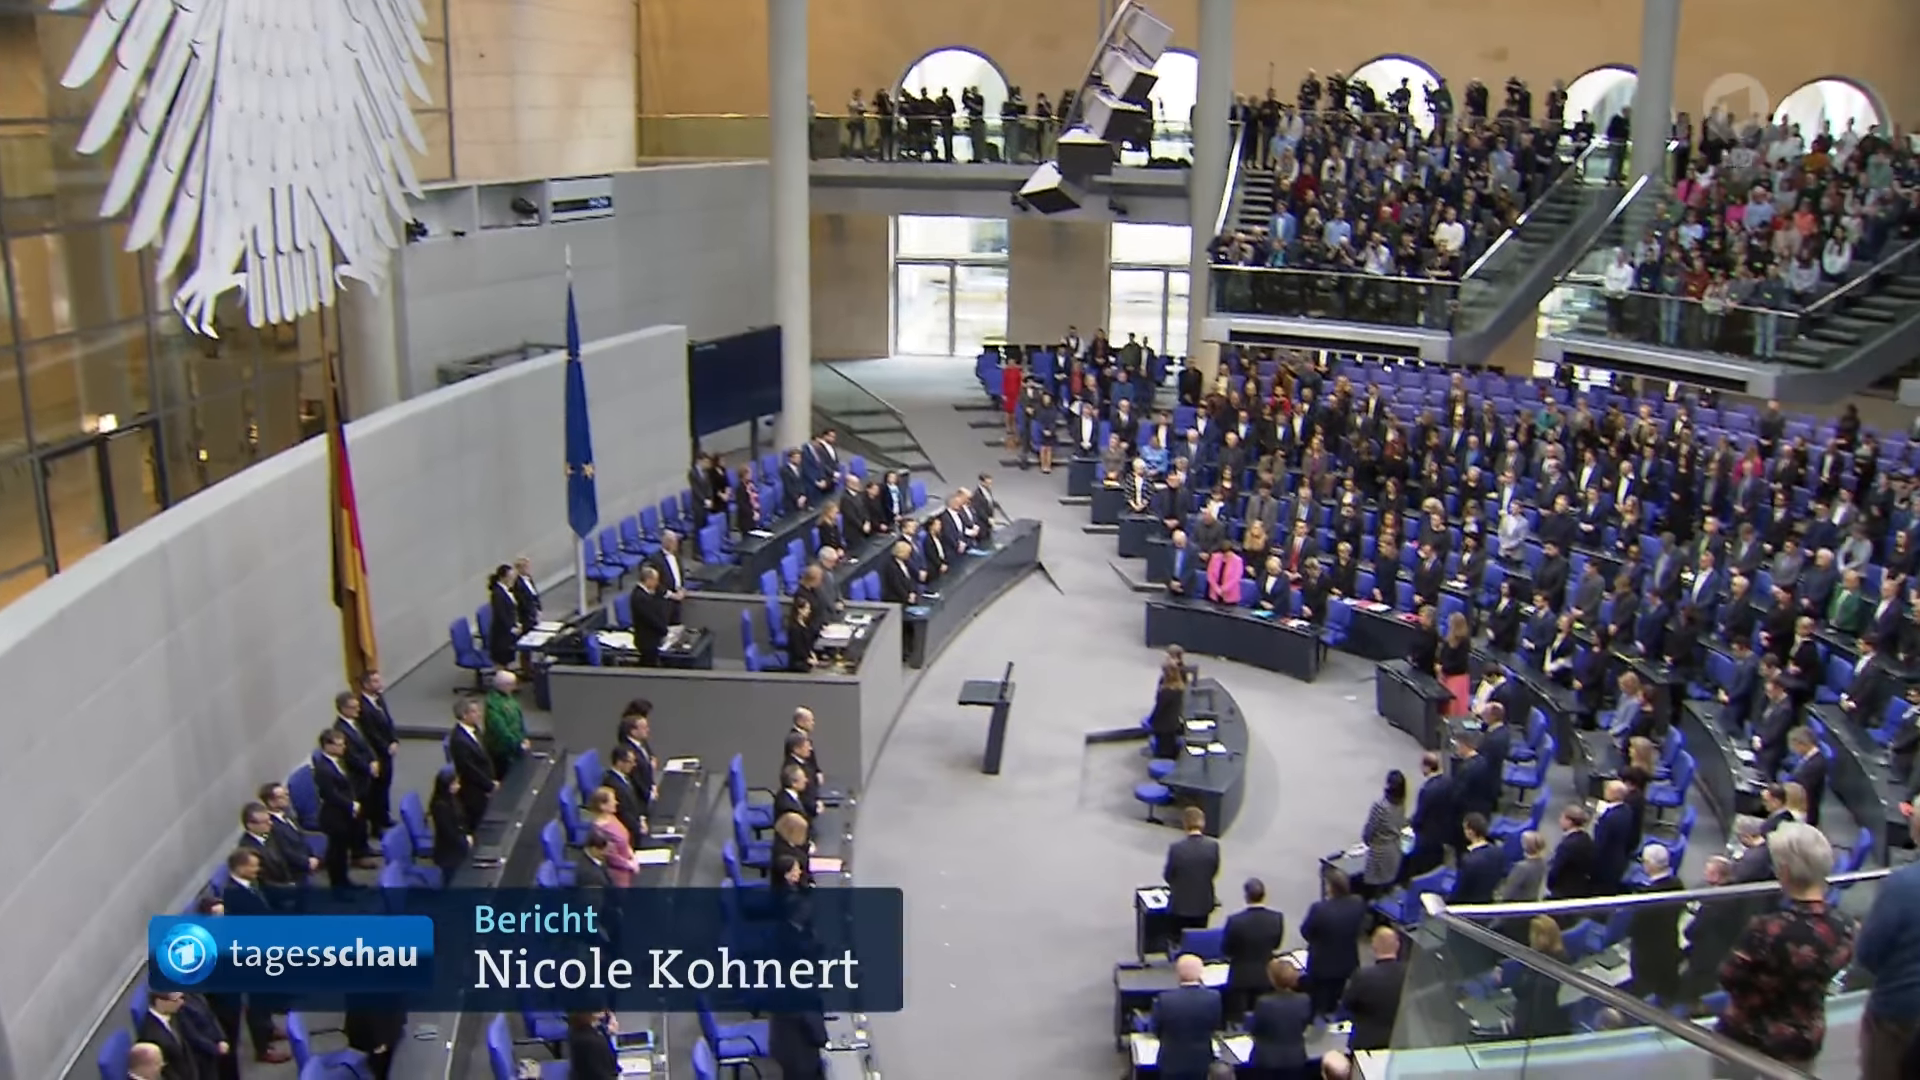
\includegraphics[width=\textwidth]{imgs/original.png}
        \caption{original}
        \label{fig:diff1}
    \end{subfigure}
    \begin{subfigure}[b]{0.48\textwidth}
        \centering
        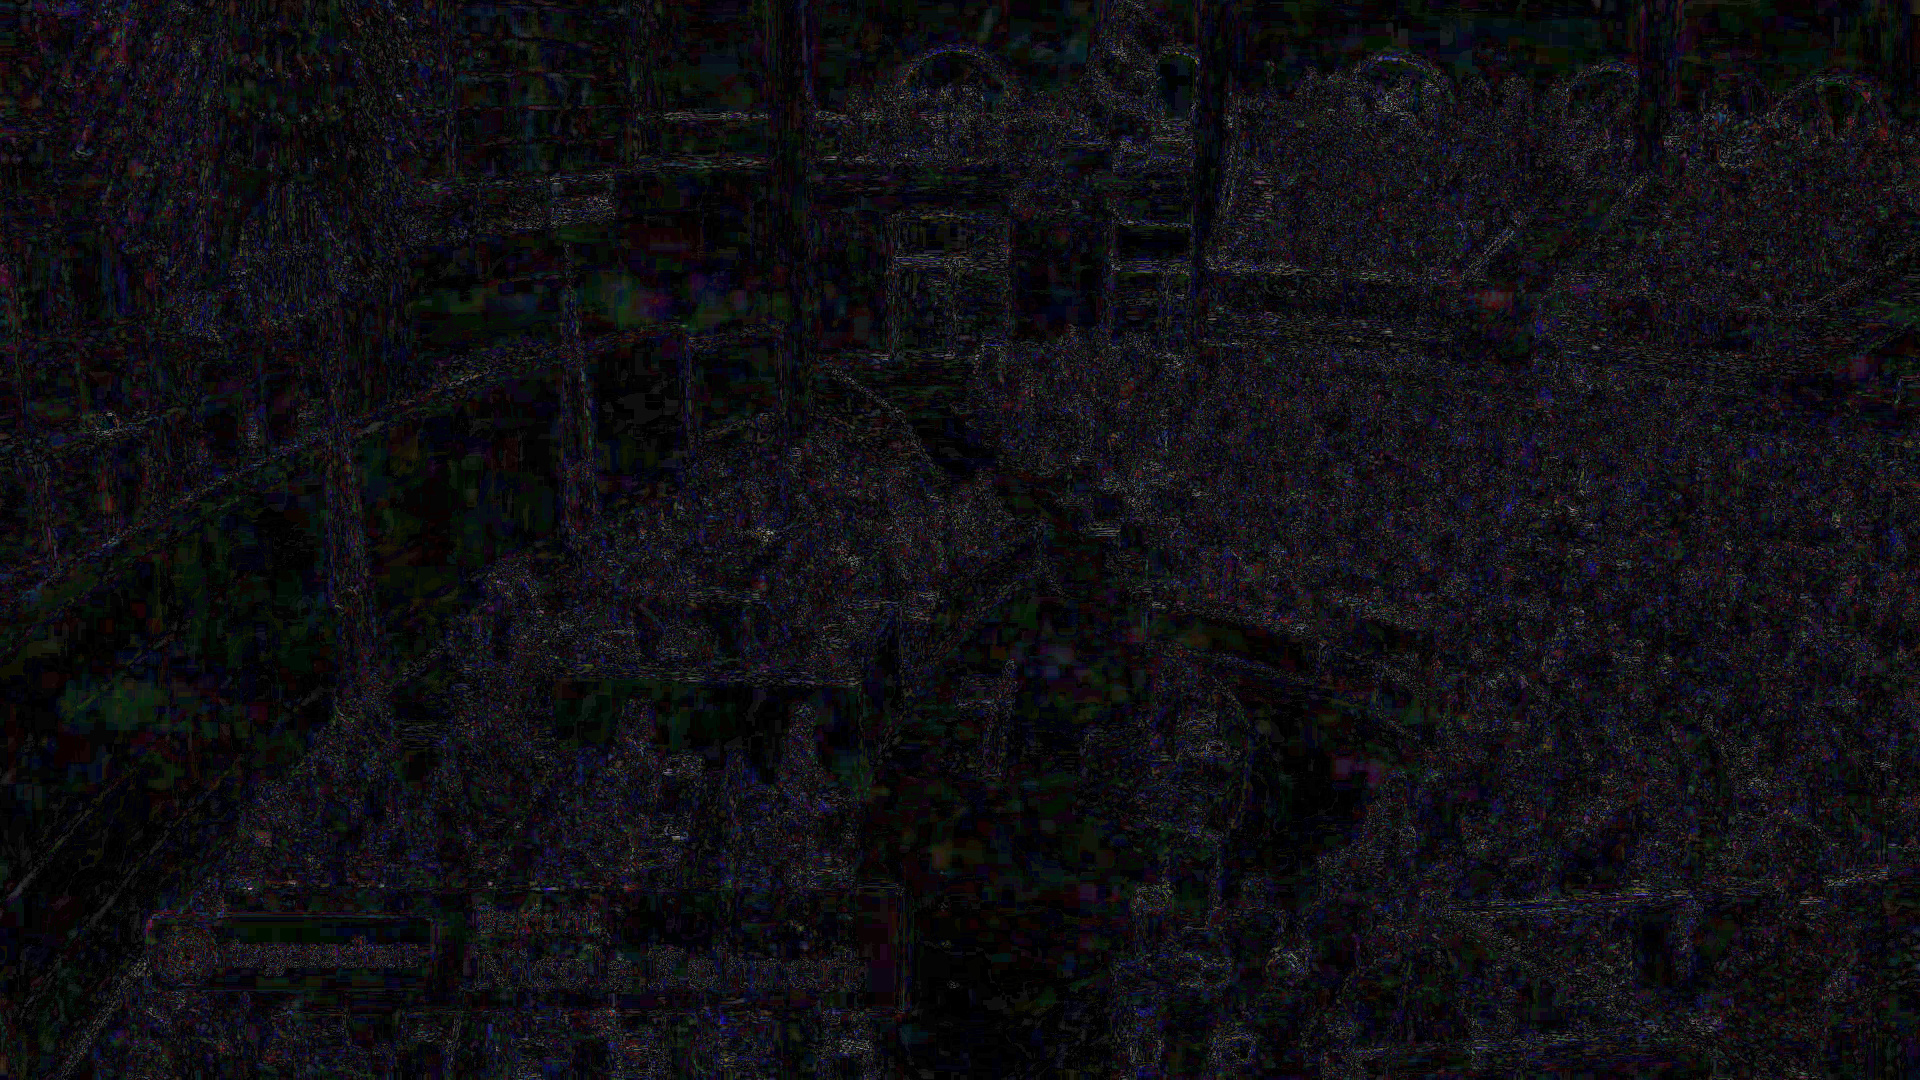
\includegraphics[width=\textwidth]{imgs/diff.jpg}
        \caption{enhanced delta}
        \label{fig:diff2}
    \end{subfigure}
    \hfill
    \caption{Comparing the unprocessed video with the watermarking delta. The magnitude of the delta has been increased for better visibility. Video by\cite{archiveTagesschauUhr}}
    \label{fig:diff}
\end{figure*}

\begin{figure*}[t]
    \centering
    \begin{subfigure}[b]{0.48\textwidth}
        \centering
        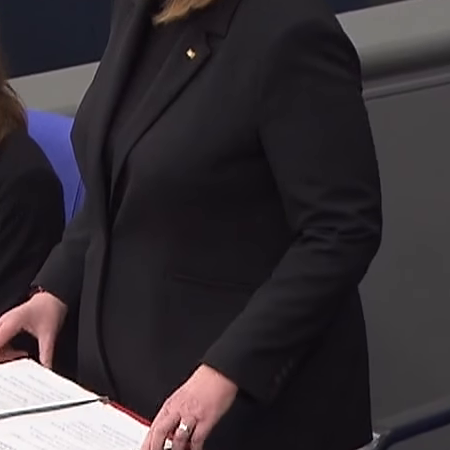
\includegraphics[width=\textwidth]{imgs/unprocessed_crop.png}
        \caption{original}
        \label{fig:dark1}
    \end{subfigure}
    \begin{subfigure}[b]{0.48\textwidth}
        \centering
        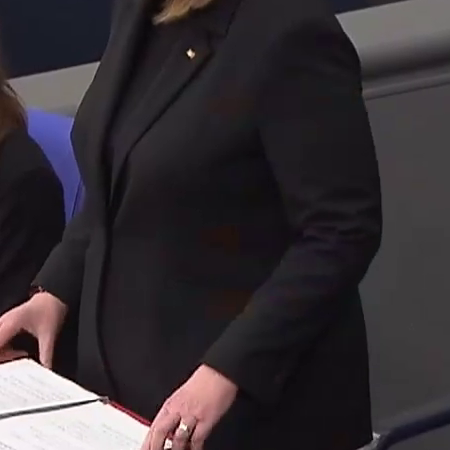
\includegraphics[width=\textwidth]{imgs/processed_crop.png}
        \caption{watermarked}
        \label{fig:dark2}
    \end{subfigure}
    \hfill
    \caption{Comparing unprocessed and watermarked image. Video by\cite{archiveTagesschauUhr}}
    \label{fig:dark}
\end{figure*}



\begin{figure*}[t]
    \centering
    \begin{subfigure}[b]{0.48\textwidth}
        \centering
        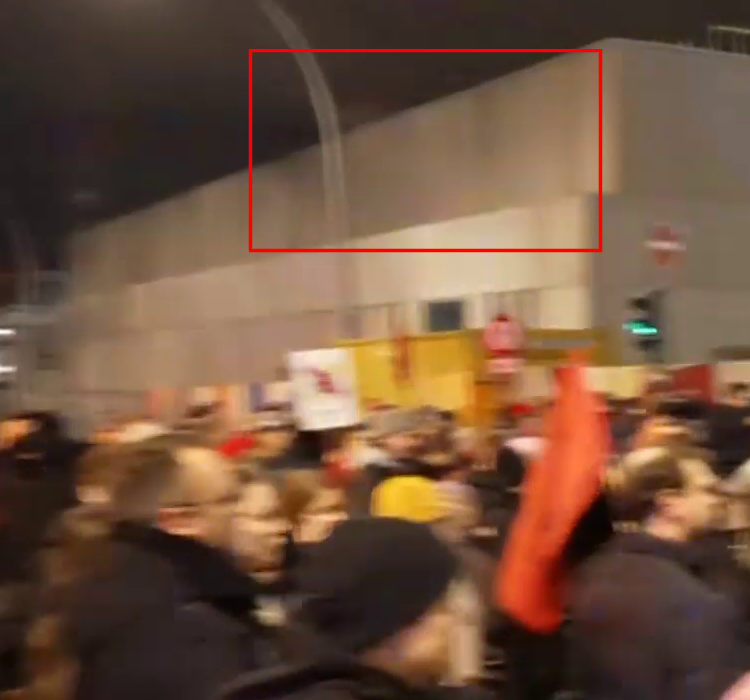
\includegraphics[width=\textwidth]{imgs/motion1_annotate.png}
        \caption{first image}
        \label{fig:motion1}
    \end{subfigure}
    \begin{subfigure}[b]{0.48\textwidth}
        \centering
        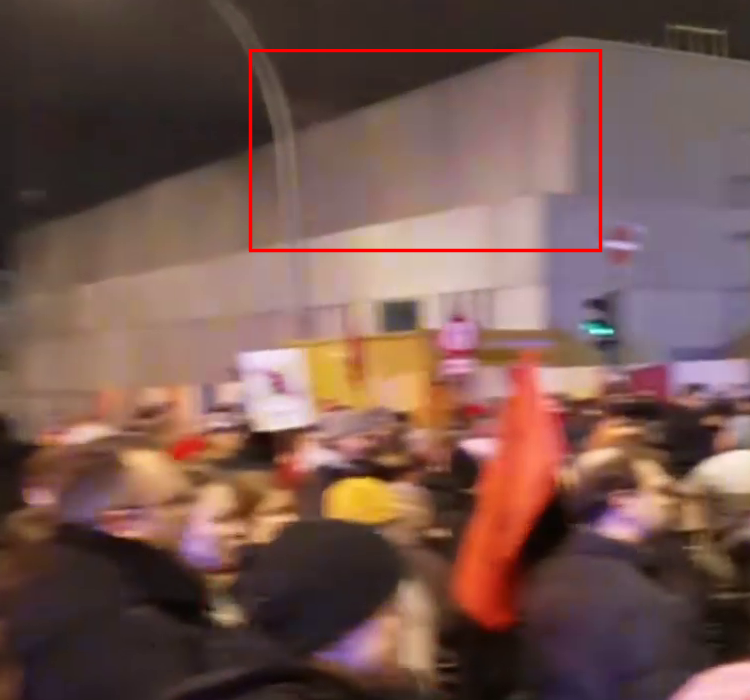
\includegraphics[width=\textwidth]{imgs/motion2_annotate.png}
        \caption{second image}
        \label{fig:motion2}
    \end{subfigure}
    \hfill
    \caption{Comparing two successive frames, with drastic changes in color. Video by\cite{archiveTagesschauUhr}}
    \label{fig:motion}
\end{figure*}

\subsection{Robustness}
I was able to verify that the watermark is able to withstand, reencoding, slight cropping and the analog bridge. It should however be noted, that in the latter cases rarely all 96 bits can be correctly recovered, typically hovering more around 90-95\% bit accuracy. Given my relatively small test library that was sufficient to correctly identify the original video. It should however be noted that larger libraries collisions are possible and might be mitigated by not just showing the user the closest match, but have them choose the correct one from a ranked list.

\section{Discussion}

While the project demonstrates the feasibility and usefulness of the concept of using watermarking for metadata recovery, additional work is required to turn it into a production-ready solution. There also remain a number of conceptual hurdles that complicate real-world adoption. The watermarking algorithm used here is open source and thus any embedded watermark can be easily spoofed. This project addresses that concern by giving the user the option to compare the videos. An improved implementation might automate this using robust perceptual comparison algorithms like VMAF~\cite{topiwala2021vmafvariantsunifiedvqa} or highlight differences in a way more obvious to the user. The fundamental issue with this approach is scalability. It requires that services, that store the database and watermarks also store the original videos. While that might be logistically feasible for large content providers and platforms, it is difficult to separate it out into its own service. Instead of storing the original video itself, a service could just store links to the original, but would then be subject to link rot. Hosters of these videos, might want to re-encode them at some point to save space, change their URL schema, might be compelled by users or legal actions to delete videos or could simply go out of business. Any such watermarking metadata service would clearly degrade over time. 
The solution typically proposed~\cite{durablecontent} is to instead of videos store perceptual hashes. The problem of perceptual hashes is that by their very nature similar things will look similar. Often times, subtle manipulation of videos can already cause a great amount of harm. Without the original video it becomes impossible to determine just from the video hash whether a video was actually manipulated and in what way or whether the metadata just got accidentally lost. At the core of the trust model behind C2PA is the cryptographic integrity of the metadata. When relying on solutions like fingerprinting or watermarking such guarantees are impossible to provide.
That adds another layer to the already difficult question of how to communicate the information and trust provided by C2PA to the user.\\
Aside from its interaction with watermarking, there are also still many question marks with regards to C2PA itself. One of the goals of C2PA was not just to make provenance of media files verifiable, but to make their creation history transparent. To that end, producers of image editing software\cite{adobe} and AI image generators\cite{openai} have begun to include C2PA into their offerings. While that works well for server-generated content, media created on the user's device would either require to be uploaded to the server, raising concerns about privacy or include the signing keys themselves making them vulnerable to extraction.
Many publishers might also prefer not to publish their editing history. While this editing history can easily be replaced by less transparent provenance information having it in the first places carry significant risk that it might get accidentally leaked.




\section{Conclusion}
I presented a approach to reinforcing media content authenticity by fusing C2PA content credentials with invisible watermarking. This method addresses the critical problem of metadata loss—a common vulnerability in provenance tracking—by embedding a persistent identifier directly into the media. My implementation using a Rust backend (with Python modules for watermark embedding and extraction) and the Video Seal watermarking model demonstrates that it is feasible to create durable watermarks for video that survive common transformations and enable post-hoc verification of origin.\\


% An example of a floating figure using the graphicx package.
% Note that \label must occur AFTER (or within) \caption.
% For figures, \caption should occur after the \includegraphics.
% Note that IEEEtran v1.7 and later has special internal code that
% is designed to preserve the operation of \label within \caption
% even when the captionsoff option is in effect. However, because
% of issues like this, it may be the safest practice to put all your
% \label just after \caption rather than within \caption{}.
%
% Reminder: the "draftcls" or "draftclsnofoot", not "draft", class
% option should be used if it is desired that the figures are to be
% displayed while in draft mode.
%
%\begin{figure}[!t]
%\centering
%\includegraphics[width=2.5in]{myfigure}
% where an .eps filename suffix will be assumed under latex, 
% and a .pdf suffix will be assumed for pdflatex; or what has been declared
% via \DeclareGraphicsExtensions.
%\caption{Simulation results for the network.}
%\label{fig_sim}
%\end{figure}

% Note that the IEEE typically puts floats only at the top, even when this
% results in a large percentage of a column being occupied by floats.


% An example of a double column floating figure using two subfigures.
% (The subfig.sty package must be loaded for this to work.)
% The subfigure \label commands are set within each subfloat command,
% and the \label for the overall figure must come after \caption.
% \hfil is used as a separator to get equal spacing.
% Watch out that the combined width of all the subfigures on a 
% line do not exceed the text width or a line break will occur.
%
%\begin{figure*}[!t]
%\centering
%\subfloat[Case I]{\includegraphics[width=2.5in]{box}%
%\label{fig_first_case}}
%\hfil
%\subfloat[Case II]{\includegraphics[width=2.5in]{box}%
%\label{fig_second_case}}
%\caption{Simulation results for the network.}
%\label{fig_sim}
%\end{figure*}
%
% Note that often IEEE papers with subfigures do not employ subfigure
% captions (using the optional argument to \subfloat[]), but instead will
% reference/describe all of them (a), (b), etc., within the main caption.
% Be aware that for subfig.sty to generate the (a), (b), etc., subfigure
% labels, the optional argument to \subfloat must be present. If a
% subcaption is not desired, just leave its contents blank,
% e.g., \subfloat[].


% An example of a floating table. Note that, for IEEE style tables, the
% \caption command should come BEFORE the table and, given that table
% captions serve much like titles, are usually capitalized except for words
% such as a, an, and, as, at, but, by, for, in, nor, of, on, or, the, to
% and up, which are usually not capitalized unless they are the first or
% last word of the caption. Table text will default to \footnotesize as
% the IEEE normally uses this smaller font for tables.
% The \label must come after \caption as always.
%
%\begin{table}[!t]
%% increase table row spacing, adjust to taste
%\renewcommand{\arraystretch}{1.3}
% if using array.sty, it might be a good idea to tweak the value of
% \extrarowheight as needed to properly center the text within the cells
%\caption{An Example of a Table}
%\label{table_example}
%\centering
%% Some packages, such as MDW tools, offer better commands for making tables
%% than the plain LaTeX2e tabular which is used here.
%\begin{tabular}{|c||c|}
%\hline
%One & Two\\
%\hline
%Three & Four\\
%\hline
%\end{tabular}
%\end{table}


% Note that the IEEE does not put floats in the very first column
% - or typically anywhere on the first page for that matter. Also,
% in-text middle ("here") positioning is typically not used, but it
% is allowed and encouraged for Computer Society conferences (but
% not Computer Society journals). Most IEEE journals/conferences use
% top floats exclusively. 
% Note that, LaTeX2e, unlike IEEE journals/conferences, places
% footnotes above bottom floats. This can be corrected via the
% \fnbelowfloat command of the stfloats package.






% if have a single appendix:
%\appendix[Proof of the Zonklar Equations]
% or
%\appendix  % for no appendix heading
% do not use \section anymore after \appendix, only \section*
% is possibly needed

% use appendices with more than one appendix
% then use \section to start each appendix
% you must declare a \section before using any
% \subsection or using \label (\appendices by itself
% starts a section numbered zero.)
%


% Can use something like this to put references on a page
% by themselves when using endfloat and the captionsoff option.
\ifCLASSOPTIONcaptionsoff
  \newpage
\fi



% trigger a \newpage just before the given reference
% number - used to balance the columns on the last page
% adjust value as needed - may need to be readjusted if
% the document is modified later
%\IEEEtriggeratref{8}
% The "triggered" command can be changed if desired:
%\IEEEtriggercmd{\enlargethispage{-5in}}

% references section

% can use a bibliography generated by BibTeX as a .bbl file
% BibTeX documentation can be easily obtained at:
% http://mirror.ctan.org/biblio/bibtex/contrib/doc/
% The IEEEtran BibTeX style support page is at:
% http://www.michaelshell.org/tex/ieeetran/bibtex/
%\bibliographystyle{IEEEtran}
% argument is your BibTeX string definitions and bibliography database(s)
%\bibliography{IEEEabrv,../bib/paper}
%
% <OR> manually copy in the resultant .bbl file
% set second argument of \begin to the number of references
% (used to reserve space for the reference number labels box)

\bibliography{bibtex/bib/IEEEabrv.bib,bibtex/bib/IEEEexample.bib}{}
\bibliographystyle{IEEEtran}

% biography section
% 
% If you have an EPS/PDF photo (graphicx package needed) extra braces are
% needed around the contents of the optional argument to biography to prevent
% the LaTeX parser from getting confused when it sees the complicated
% \includegraphics command within an optional argument. (You could create
% your own custom macro containing the \includegraphics command to make things
% simpler here.)
%\begin{IEEEbiography}[{\includegraphics[width=1in,height=1.25in,clip,keepaspectratio]{mshell}}]{Michael Shell}
% or if you just want to reserve a space for a photo:

% You can push biographies down or up by placing
% a \vfill before or after them. The appropriate
% use of \vfill depends on what kind of text is
% on the last page and whether or not the columns
% are being equalized.

%\vfill

% Can be used to pull up biographies so that the bottom of the last one
% is flush with the other column.
%\enlargethispage{-5in}



% that's all folks
\end{document}


